\section{Methodology}
\subsection{Acquisition of the datasets}
The LIDC/IDRI database consists of 1018 thoracic CT scans that are obtained from
a heterogeneous range of scanner models (seven GE Medical Systems LightSpeed
scanner models, four Philips Brilleance scanner models, five Siemens Definition,
Emotion, and Sensation scanner models and one Toshiba Aquilion scanner model).
The database includes only one scan per patient so the scans are not correlated.
The nodules in the scans were delineated by at least four different expert
radiologists to identify as much nodules as possible. For this purpose the
indentification process was also subdivided into two phases: a blinded read
phase and an unblinded read phase. During the initial blinded read phase each
radiologist independently reviewed all scans and indicated the nodules in the
range of 3 to 30 mm and nodules smaller than 3 mm (if not clearly benign).
In the subsequent unblinded read phase the anonymized blinded read results of
all radiologists were revealed to each of the radiologists who then
independently reviewed their marks along with the anonymous marks of their
colleagues. The delineation of the nodules was done completely manually or in a
semiautomated way. This was allowed as a study on this topic showed that the
variation in nodule delineation done by different radiologists substantially
exceeded the variation derived from different software tools \cite{lidcbase}.

50 CT scans were obtained from the LIDC database \footnote{Freely available
at \url{http://cancerimagingarchive.net}.}. 12 scans were removed as they only
contained 1-voxel nodules. The pixel size of the scans varied between 0,586 and
0,963 mm and the slice thickness varied between 1,25 or 2,50 mm. This means the
diameter of the annotated 1-voxel nodules was less than 1 mm (micronodules).
These nodules are difficult to detect for a radiologist, especially if they are
hidden in a maze of vessels of the same magnitude. Therefore, some databases do
not require the radiologist to mark such small findings. In the Nelson Trail
database for example the radiologists do not have to mark nodules of which the
volume calculated by the Siemens LungCARE workstation software is less than 15
$mm^3$ \cite{mur}. This volume corresponds to a sphere with a diameter of about
3 mm, which is obviously more the 1 mm diameter from our 1-voxel nodules.
In the LIDC/IDRI database there were no limitations set on the diameters of the
nodules to be marked. However, the chance the radiologists marked every single
micronodule is very small. The training of the CAD algorithm can therefore not
be done properly as the annotations of the datasets are most propably incomplete
for nodules with a diameter less than 1 mm. Therefore, the datasets containing
only 1-voxel micronodules and the annotations of 1-voxel nodules in the
remaining datasets were removed. Furthermore, focussing on the detection of
these micronodules limits the level of thresholding that can be performed during
the classification of the datasets. Retaining these micronodules would prevent
us from eliminating a substantial part of the false positive findings. So
after eliminating these 38 scans remained for training and testing.
The RF algorithm was trained and validated on 30 and 8 CT scans respectively,
consisting of 5168 and 1249 slices with a average of 172 and 156 slices per
scan. Together with the original DICOM images the associated XML files
were obtained. These XML files provided a set of characteristics for each nodule
found: region, subtlety, spiculation, internal structure, lobulation, shape
(sphericity), solidity, margin, and likelihood of malignancy \cite{lidcbase}.
The trainingsdataset contained 64 nodules with each nodule containing 150 voxels
on average. The minimum and maximum radii of the annotated nodules was 2 mm and
18 mm respectively. The testdataset contained 19 nodules.


\subsection{Preprocessing of the data} %TODO this isn't preprocessing..
The initial exploration of the data and the generation of a mask to perform a
lung segmentation were done in MeVisLab 2.5.1 (VC11-64) (MeVis Medical Solutions
AG, Bremen, Germany). Further processing of the data and the implementation of
the RF algorithm were carried out in Python 2.7.6 (Python Software Foundation,
Delaware, U.S.A).  The training and testing of the RF based algorithm was
performed on a computer with Intel Core2 DUO CPU (2,27 GHz) and 3 GB of RAM.
Training the algorithm on 30 scans took 1 hour and 50 minutes. The processing of
a new medium large dataset (136 slices) takes about 10 minutes.

\subsubsection{Processing of the annotations}
%convention: x,y,z = pixel, X,Y,Z = world

The annotations were partially provided in pixel coordinates -- x and y values
-- and partially in world coordinates -- Z values -- so the Z coordinates were
converted into pixel coordinates to find the nodule regions. The annotations
contained a list of x and y coordinates to indicate the position of each pixel
belonging to the contour of each nodule per slice. From these coordinates the
center of gravity plus the minimum and maximum radius of each nodule was
calculated per slice. The 1-voxel nodules were removed from the list of
annotations. In the rest of the algorithm each nodule was represented by its
center of gravity and its minimum radius.

\subsubsection{Lung segmentation}
It was assumed that, if the whole 3D scan was fed to the cascaded classifier,
only the soft tissue would remain after the first cascade. The grey value of
each voxel was used as a feature on this first level. Unfortunately, this method
did not prove to be efficient, so a second option was taken into consideration:
a proper lung segmentation as a preprocessing step.

By performing a lung segmentation, the amount of voxels that have to be
processed further on is significantly reduced by about 85\%. Furthermore, it has
the advantage that the soft tissues outside the lungs are eliminated so the
accuracy of the nodule detection system is increased. Therefore, it is the first
step that is performed in a lot of papers \cite{keshani, elbaz, teramoto}. We
started with implementing a lung segmentation algorithm based on \cite{keshani}.
The first part of this algorithm consists of obtaining a binary lung CT image by
adaptive fuzzy thresholding. In the binary image the lungs and the background
are separated from the soft tissues of the body.
Then two windows of different sizes are applied to close all the gaps in the
mask and the initial lung mask is obtained by sweeping a rotated window over the
entire binary image.
This sweeping is necessary to transfer non-isolated nodules into isolated ones.
Finally the mask is used to initiate an active contour model automatically for
segmenting the lung area. As stated the first step of this algorithm was
supposed to provide us with a variable, but accurate threshold to make the
binary image. The performance of this first step was assessed by applying the
algorithm on 42 slices -- 28 slices with lungs and 14 without lungs -- equally
distributed over 7 scans. The results varied among the scans. In some cases the
algorithm selected the appropriate threshold, in other cases the soft tissue
around the lungs was not eliminated well. Furthermore, performing the lung
segmentation as was described above would take a considerable amount of time
(minutes). Instead, a fixed threshold of 1600 was empirically established to
perform a body segmentation and to separate the soft body tissues from the rest
of the image. This is permitted because CT scanners have a carefully calibrated
output. Then gaps (lungs) in the body mask were closed by hole filling so a mask
of the entire body was obtained. As this body segmentation already eliminated
55\% of all voxels and no complex calculations had to be done to obtain the
binary image, this result was found satisfying enough.

% TODO tabel met experimenten om vaste threshold te bepalen er nog inzetten?
Despite the reduced amount of voxels, applying the algorithm still raised memory
errors depending on the dimensions of the scan.
In order to reduce the amount of voxels even further in the pre-processing
phase, a full lung segmentation was performed in a semiautomatic way in
MeVisLab. After the scans were loaded in MeVisLab, the user manually indicates
three points inside the lung area. Based on these points region growing is
performed and a binary mask for the lung area is generated. The gaps in the
binary mask -- which represent nodules in the lung area and nodules hidden in
the lung wall -- are closed by dilation. This mask is then exported to Python
for further processing of the images. 

An alternative way of performing a lung segmentation in Python would be
calculating the body mask at the fixed threshold of 1600 and subtracting this
mask from a similar mask in which the lung gaps are closed. In this way only the
lung area is retained. Then a dilation and erosion should be performed as well
to include the nodules hidden in the lung wall.

\subsection{Training of the classifier}
\subsubsection{Preparation of the training dataset}
Based on the associated annotations the center of gravity, the minimum and
maximum radius of each nodule was calculated. With this information a sphere
was constructed which comprised the whole nodule. To select the central volume
of the nodule, one third of the radius was taken as an artificial boundary. Only
the voxels in this center were considered further in the process as voxels
belonging to a nodule. Reducing the amount of positive voxels -- voxels
comprised by a nodule -- was done to avoid taking into account the ambiguous
edges of the nodules. These edges might confuse the classifier. As the aim of
this project was not to delineate entire nodules but assigning nodule
probabilities to the voxels in the image, this reduction in order to provide
clear training data for the classifier was justified.

However, instead of a sphere -- which defines the nodules in 3D -- this concept
was applied per slice as it was noticed that the delineation of the nodules was
not always done properly so a lot of nodules showed a flattened shape
(\autoref{fig:flatNodule}).
Therefore, the minimum radii of the nodule in each slice were separately
determined and two third of these radii was taken to select the central volume
of the nodule. A list of positive voxels per scan was constructed this way.
\begin{figure}[htp]
 \begin{center}
    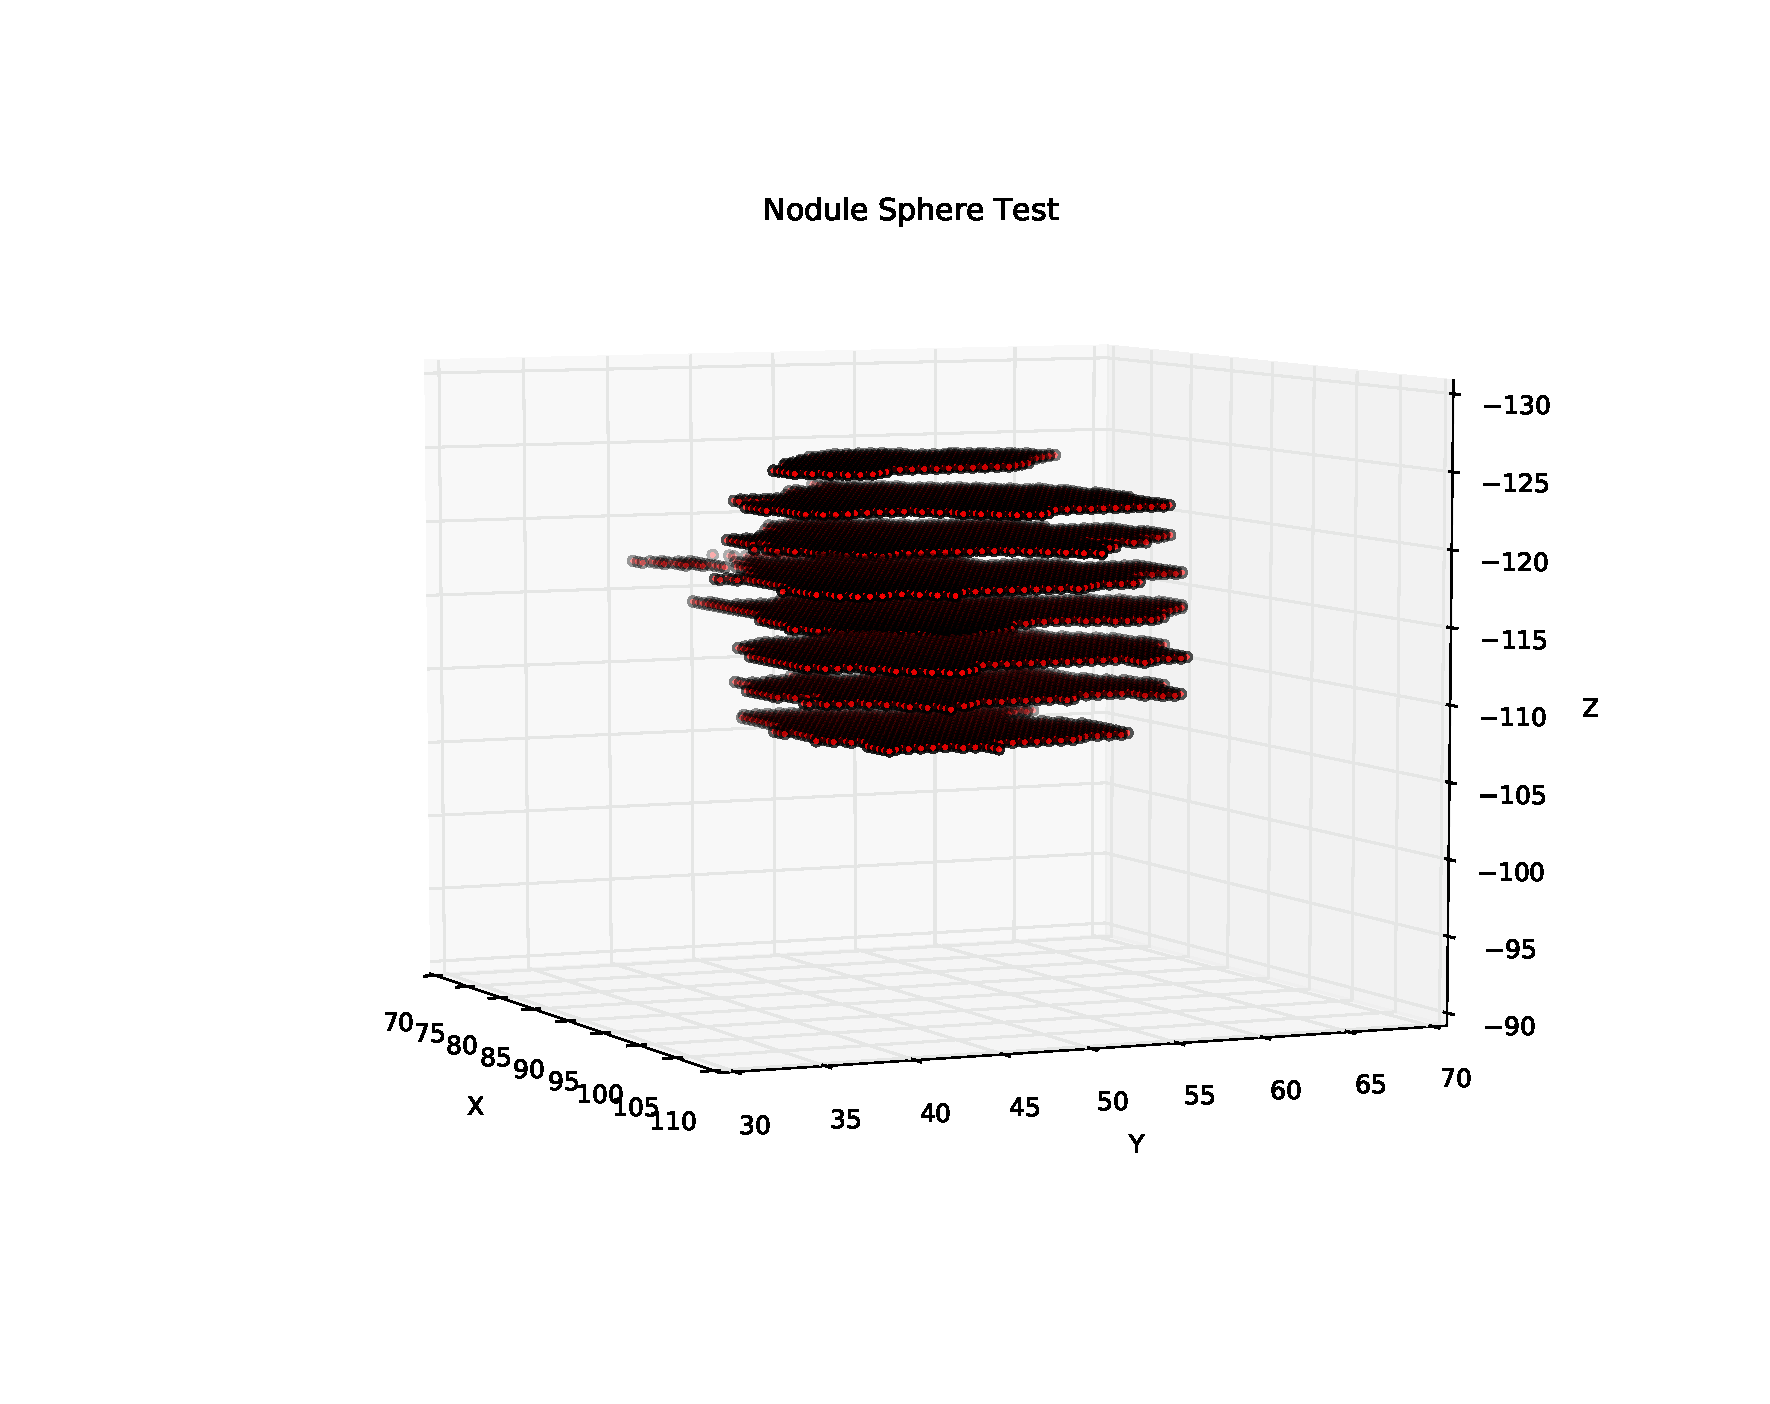
\includegraphics[width=\linewidth]{img/NoduleSphereTest_0001.pdf}
    \caption{Flattened shape of nodule (LIDC scan 0001)}
    \label{fig:flatNodule}
 \end{center}
\end{figure}

To train a classifier, a list of positive and negative
examples are necessary. Therefore, a second list of voxels was constructed. The
amount of voxels was taken the same as in the list of positive voxels to obtain
a balanced training dataset. The positions of the negative voxels were selected
at random over the entire image. The only constraint was that they were not
allowed the be situated within two times the maximum radius of each nodule. This
constraint was imposed to avoid ambigous training data.

Then features were calculated for both the positive and the negative voxels. The
features that were used are discussed in section \ref{sec:featureExtraction}.
This resulted in a list of features and a class (nodule or non-nodule) per
voxel. This whole process was repeated for all scans and the results were then
concatenated to obtain a dataset to train the ensemble classifier. We summarized
it using pseudocode in algorithm \ref{alg:train}.

\begin{algorithm}[htp]
	\DontPrintSemicolon
	\caption{Training Phase\label{alg:train}}
	\ForEach{$dataset \in trainingsets$}{
		load DICOM files\;
		load XML annotations\;
		\ForEach{$nodule \in annotations$}{
			\ForEach{$slice \in nodule$}{
				select positive voxels ($d < 0.66R_{min}$)
			}
		}
		\While {negative pixels $<$ positive pixels}
		{	select random pixel in volume\;
			\If{not near nodules ($d > 2R_{max}$)}{
				select negative voxel
			}
		}
	}
	\For{level from 1 to max}{
		\ForEach{selected pixel}{
			generate feature vectors up to level\;
		}
		train classifier\;
		save classifier model\;
	}
\end{algorithm}

\subsubsection{Feature extraction and selection} \label{sec:featureExtraction}
\paragraph{Features implemented in final algorithm}
The \textbf{grey value} of each voxel is the only feature of the cascaded
classifier at level one. From this, the classifier learns that nodules are
always part of the soft tissue window. When asked to identify nodules with this
information alone, the classifier will simply highlight all soft tissue in the
image. Remember that during the preprocessing we applied a lung mask. Hence all
soft tissue outside of the lungs -- save for a thin edge caused by dilation --
is already discarded. By combining the two results, we are left only with thin
lung edges, nodules and bronchi/bronchioli. The task of the next classifiers in
the cascade will be to further distinguish between these different structures.

In level two, our focus goes to discarding the remaining lung edges and
highlighting the nodules. We do this by combining a LoG \textbf{blob detector}
with a \textbf{distance map}. As explained in section \ref{sec:laplace_theory},
the LoG operator is very good in detecting light blobs on a darker background
such as nodules. The remaining lung edges in contrast do not fit this
description at all. To find out which sigma would work best, we performed a
couple of tests. First, we know that larger sigmas work better on larger nodules
and vice versa. To that end, we searched for the smallest and largest nodule
over all our datasets. Next, we empirically established the sigmas that yielded
the best results for each. Because we do not know ahead of time how big the
nodule we have to detect will be, we calculate the LoG for all intermediary
values. The results of our test show that nodules radii lie roughly between
\ldots mm and \ldots mm and that we need sigmas between 2mm and 10mm to cover
this range.
% TODO graph sven radii

To make the difference even more clear to the classifier, a distance map was
calculated based on the original lung mask. Alternatively, one could also work
with an ordinary edge detector, e.g. sobel. By blurring that output with a
Gaussian, we get a similar distance-to-edge feature. However, we chose the
distance map over this approach because it simply contained more information. Of
course we can't blindly discard any voxels too close to the edges, because
nodules can be closeby as well. That is why a distance map alone is not enough.

At the third and fourth level \textbf{3D averaging} was implemented to get rid
of the bronchi and bronchioles that were still present. See section
\ref{sec:3davg} for more information. With the help of all the features above,
the classifier should have enough information to separate the nodules from other
structures in and around the lung.

\paragraph{Experimental features}
This paragraph provides an overview of other features that were
tested but that were not implemented in the final classifier because of several
reasons.

The \textbf{skewness and kurtosis} of a 3D window around each
voxel was calculated as a measure for the texture of a certain part of the image. The
skewness is a measure of the asymmetry of the probability distribution
distribution of a real-valued random variable (grey value) about its mean. The
kurtosis is a measure of the peakedness of the probability distribution of a
real-valued random variable. However, the implementation of these first order
statistics in the final classifier was prohibited by the time needed (hours) to
calculate these features for every voxel in the image.

Another obvious feature, apart from the grey value of each voxel, is the
\textbf{position} $(X, Y, Z)$ of each voxel in the 3D image. An even better
feature is the \textbf{relative position} $(\tfrac{X}{X_{max}}, \tfrac{Y}{Y_{max}}, \tfrac{Z}{Z_{max}})$ as
it takes into account that the size of the datasets might change. However, after
testing it appeared that these features would only be useful if a very large
amount of training data was used. The training set had to be large enough so
almost every possible nodule position inside the lungs was covered by the
training data. As it is very difficult to estimate how many scans are needed for
this purpose and training on this large amount of data would take a lot of time,
the feature 'position' and 'relative position' were exluded from the feature set.
Instead a distance map based on the lung mask was implemented as a feature.

A \textbf{3D Sobel filter} for edge detection was implemented as well. A Sobel
filter is typically a $3 \times 3$ convolution mask that approximates the
partial derivative of an image along an axis. The results of multiple sobel
filters can be combined to calculate the gradient magnitude of each pixel. A
high magnitude usually corresponds with an edge in the original image.

To be really useful in nodule detection, the distance from each voxel to
neighbouring edges had to be calculated. However, due to a lack of time this was
not feasible anymore. Instead, the distance map mentioned above was used as a
substitute.

The \textbf{entropy} of an image is a measure for the chaos of the image in a
certain neighbourhood. Low entropy images are images where vast areas of pixels
have the same grey values. Images with high entropy show a large contrast
between neighbouring pixels. Therefore, it is a measure for the texture of an
image. The entropy of the entire 3D image was calculated and then the values for
each voxel were extracted. However, the time demand for these calculations were
far from negligible and as a consequence this feature was eliminated again.

A feature \textbf{neighbours} calculated the sum, the subtraction, the
multiplication and the quotient of the voxel in front and behind, left and right
and above and below a target voxel. Each of these operations where also
performed with the target voxel itself and the neighbouring voxel. Another
substantial amount of features were based on calculations within \textbf{3D
windows} that were swept over the lung mask of the image. The same operations
as in neighbours were executed on a larger scale: the neigbouring voxels were
determined by a certain adaptable window around the target voxel. Except for
these basic operations the mean, the standard variance, the minimum and the
maximum of the grey values of each window were calculated. Then these parameters
and the grey value of the target voxel were used for performing the basic
operations (sum, subtraction, multiplication, quotient) on. The same idea was
applied on the rows and columns in each window. The mean of different rows and
columns were determined and compared to each other by means of summing them up,
subtracting them, dividing one by another and multiplying them. In these windows
a frequency count was performed for each grey value in the window. These
frequencies were again compared. The results that were obtained this way could
be compared to one another by comparing the results for subwindows within larger
windows or within the entire image. However, none of these features were
implemented in the final classifier as calculating features for each individual
voxel in an image took too much time (hours).

%\subsubsection{Training of the classifier}
\subsubsection{Cross validation}
During the training phase, we already want to get an idea about the future
performance of our classifier. Of course we could use the whole feature set in
the training, and use the same features afterwards to check if our classifier is
performing well. However, this is considered a form of cheating, and the test
would not tell us much about the predictive power of the classifier on new data.
That is why it is important to reserve a fraction of the feature vectors for
cross validation. A strategy called stratified K-fold is used to repeatedly
split the feature set randomly in a train and a test fraction.
The stratified adjective means that the proportion of nodules to non-nodules are
similar in both fractions. Each time -- also called \textit{fold} -- the
classifier is trained with the train fraction and performance is checked with
the test fraction. After a number of folds, these results are combined to give a
proper estimate of the classifier performance in terms of accuracy (or other
score metric).

This cross validation can also be used to determine the optimal hyperparameters
of the classifier. By generating a grid of parameters and corresponding value
ranges, all combinations can be tested, and the one with the highest score can
be retained. In case of RF, it is important to configure it in such a way that
overfitting does not occur. This can be done by increasing either the tree
depth, the minimum number of samples per leaf or the minimum number of samples
before a split occurs. The minimum number of samples per leaf was chosen to
perform the optimalisation with.

\subsection{Testing and validation of the classifier}
From the previous section, we obtained a trained RF model that can be used to
predict the class of new image features with a certain probability. We use this
facility for two purposes: feature effectiveness testing and output validation.
But before any of that can be done, features must be calculated for all
remaining voxels in the new dataset. A cascading approach allows us to do this
while keeping computational en memory cost acceptable. Additionally, a lung mask
is applied to the whole volume, allowing us to ignore any outside voxels from
the start.

To assess feature effectiveness, we ask ourselves the following question. Is a
substantial amount of non-nodule voxels removed from the dataset without
removing the nodule voxels as well, i.e. did the specificity increase without
affecting the sensitivity? If this is the case the feature is kept at that
level, otherwise another feature is implemented. The assessment is performed
based on a probability image that is generated by combining the resulting
probability output from all feature vectors. The first section of algorithm
\ref{alg:test} summarizes this procedure.

\begin{algorithm}[htp]
	\DontPrintSemicolon
	\caption{Testing \& Validation Phase\label{alg:test}}
	\ForEach{$dataset \in testsets$}{
		load DICOM files\;
		mask $\longleftarrow$ load lung mask\;
		\For{level from 1 to max}{
			load classifier model\;
			\ForEach{$pixel \in mask$}{
				generate feature vector\;
				probability $\longleftarrow$ classify\;
			}
			combine into probability image\;
			mask $\longleftarrow$ (prob. image $>$ threshold)\;
		}
		result = mask\;
		discard non-nodule voxels ($p < 50$\%)\;
		cluster remaining voxels\;
		load XML annotations\;
		\ForEach{$nodule \in annotations$}{
			\eIf{any cluster $\in$ nodule ($d < 1.5R_{max}$)}{
				$TP{+}{+}$\tcc*[r]{nodule detected}
				delete clusters\;
			}{
				$FN{+}{+}$\tcc*[r]{nodule not detected}
			}
		}
		\ForEach{remaining cluster}{
			$FP{+}{+}$\tcc*[r]{spurious cluster}
		}
		calculate statistics
	}
\end{algorithm}

When all features are decided upon, we validate the entire algorithm by
calculating some statistics and comparing them to the state of the art in the
literature. %TODO continue

\begin{enumerate}
\item stappen die doorlopen worden + fig
\item welke algorithmes gebruikt + wat doen ze + waarom die keuze?
\item vergelijken keuzes met literatuur/commerciele systemen?
\end{enumerate}